% 2015_jiangsu_q22_fig1: 四棱锥 P-ABCD, Q在PB上
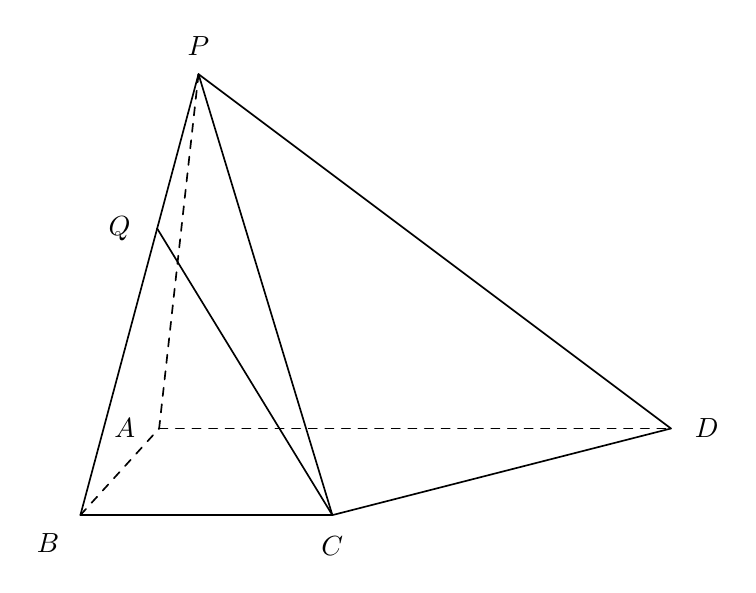
\begin{tikzpicture}[line width=0.6pt, line join=round, line cap=round, font=\normalsize]
\coordinate (P) at (1.5,6);
\coordinate (A) at (1,1.5);
\coordinate (B) at (0,0.4);
\coordinate (C) at (3.2,0.4);
\coordinate (D) at (7.5,1.5);
\coordinate (Q) at (0.975,4.04);
% 底面
\draw (B) -- (C);
\draw (C) -- (D);
\draw[dashed] (A) -- (D);
\draw[dashed] (B) -- (A);
% 侧棱
\draw (P) -- (Q);
\draw (Q) -- (B);
\draw (P) -- (C);
\draw (P) -- (D);
\draw[dashed] (P) -- (A);
% 动点连线
\draw (Q) -- (C);
% 标签(避碰外置)
\node[above, yshift=3pt] at (P) {$P$};
\node[left, xshift=-5pt] at (A) {$A$};
\node[below left, xshift=-4pt, yshift=-3pt] at (B) {$B$};
\node[below, yshift=-4pt] at (C) {$C$};
\node[right, xshift=5pt] at (D) {$D$};
\node[left, xshift=-6pt] at (Q) {$Q$};
\end{tikzpicture}
